\documentclass[1p]{elsarticle_modified}
%\bibliographystyle{elsarticle-num}

%\usepackage[colorlinks]{hyperref}
%\usepackage{abbrmath_seonhwa} %\Abb, \Ascr, \Acal ,\Abf, \Afrak
\usepackage{amsfonts}
\usepackage{amssymb}
\usepackage{amsmath}
\usepackage{amsthm}
\usepackage{scalefnt}
\usepackage{amsbsy}
\usepackage{kotex}
\usepackage{caption}
\usepackage{subfig}
\usepackage{color}
\usepackage{graphicx}
\usepackage{xcolor} %% white, black, red, green, blue, cyan, magenta, yellow
\usepackage{float}
\usepackage{setspace}
\usepackage{hyperref}

\usepackage{tikz}
\usetikzlibrary{arrows}

\usepackage{multirow}
\usepackage{array} % fixed length table
\usepackage{hhline}

%%%%%%%%%%%%%%%%%%%%%
\makeatletter
\renewcommand*\env@matrix[1][\arraystretch]{%
	\edef\arraystretch{#1}%
	\hskip -\arraycolsep
	\let\@ifnextchar\new@ifnextchar
	\array{*\c@MaxMatrixCols c}}
\makeatother %https://tex.stackexchange.com/questions/14071/how-can-i-increase-the-line-spacing-in-a-matrix
%%%%%%%%%%%%%%%

\usepackage[normalem]{ulem}

\newcommand{\msout}[1]{\ifmmode\text{\sout{\ensuremath{#1}}}\else\sout{#1}\fi}
%SOURCE: \msout is \stkout macro in https://tex.stackexchange.com/questions/20609/strikeout-in-math-mode

\newcommand{\cancel}[1]{
	\ifmmode
	{\color{red}\msout{#1}}
	\else
	{\color{red}\sout{#1}}
	\fi
}

\newcommand{\add}[1]{
	{\color{blue}\uwave{#1}}
}

\newcommand{\replace}[2]{
	\ifmmode
	{\color{red}\msout{#1}}{\color{blue}\uwave{#2}}
	\else
	{\color{red}\sout{#1}}{\color{blue}\uwave{#2}}
	\fi
}

\newcommand{\Sol}{\mathcal{S}} %segment
\newcommand{\D}{D} %diagram
\newcommand{\A}{\mathcal{A}} %arc


%%%%%%%%%%%%%%%%%%%%%%%%%%%%%5 test

\def\sl{\operatorname{\textup{SL}}(2,\Cbb)}
\def\psl{\operatorname{\textup{PSL}}(2,\Cbb)}
\def\quan{\mkern 1mu \triangleright \mkern 1mu}

\theoremstyle{definition}
\newtheorem{thm}{Theorem}[section]
\newtheorem{prop}[thm]{Proposition}
\newtheorem{lem}[thm]{Lemma}
\newtheorem{ques}[thm]{Question}
\newtheorem{cor}[thm]{Corollary}
\newtheorem{defn}[thm]{Definition}
\newtheorem{exam}[thm]{Example}
\newtheorem{rmk}[thm]{Remark}
\newtheorem{alg}[thm]{Algorithm}

\newcommand{\I}{\sqrt{-1}}
\begin{document}

%\begin{frontmatter}
%
%\title{Boundary parabolic representations of knots up to 8 crossings}
%
%%% Group authors per affiliation:
%\author{Yunhi Cho} 
%\address{Department of Mathematics, University of Seoul, Seoul, Korea}
%\ead{yhcho@uos.ac.kr}
%
%
%\author{Seonhwa Kim} %\fnref{s_kim}}
%\address{Center for Geometry and Physics, Institute for Basic Science, Pohang, 37673, Korea}
%\ead{ryeona17@ibs.re.kr}
%
%\author{Hyuk Kim}
%\address{Department of Mathematical Sciences, Seoul National University, Seoul 08826, Korea}
%\ead{hyukkim@snu.ac.kr}
%
%\author{Seokbeom Yoon}
%\address{Department of Mathematical Sciences, Seoul National University, Seoul, 08826,  Korea}
%\ead{sbyoon15@snu.ac.kr}
%
%\begin{abstract}
%We find all boundary parabolic representation of knots up to 8 crossings.
%
%\end{abstract}
%\begin{keyword}
%    \MSC[2010] 57M25 
%\end{keyword}
%
%\end{frontmatter}

%\linenumbers
%\tableofcontents
%
\newcommand\colored[1]{\textcolor{white}{\rule[-0.35ex]{0.8em}{1.4ex}}\kern-0.8em\color{red} #1}%
%\newcommand\colored[1]{\textcolor{white}{ #1}\kern-2.17ex	\textcolor{white}{ #1}\kern-1.81ex	\textcolor{white}{ #1}\kern-2.15ex\color{red}#1	}

{\Large $\underline{12a_{0829}~(K12a_{0829})}$}

\setlength{\tabcolsep}{10pt}
\renewcommand{\arraystretch}{1.6}
\vspace{1cm}\begin{tabular}{m{100pt}>{\centering\arraybackslash}m{274pt}}
\multirow{5}{120pt}{
	\centering
	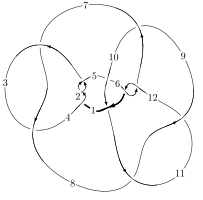
\includegraphics[width=112pt]{../../../GIT/diagram.site/Diagrams/png/1630_12a_0829.png}\\
\ \ \ A knot diagram\footnotemark}&
\allowdisplaybreaks
\textbf{Linearized knot diagam} \\
\cline{2-2}
 &
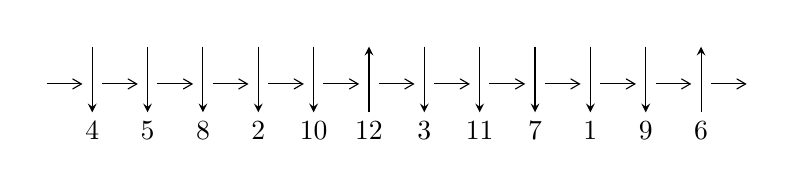
\begin{tikzpicture}[x=20pt, y=17pt]
	% nodes
	\node (C0) at (0, 0) {};
	\node (C1) at (1, 0) {};
	\node (C1U) at (1, +1) {};
	\node (C1D) at (1, -1) {4};

	\node (C2) at (2, 0) {};
	\node (C2U) at (2, +1) {};
	\node (C2D) at (2, -1) {5};

	\node (C3) at (3, 0) {};
	\node (C3U) at (3, +1) {};
	\node (C3D) at (3, -1) {8};

	\node (C4) at (4, 0) {};
	\node (C4U) at (4, +1) {};
	\node (C4D) at (4, -1) {2};

	\node (C5) at (5, 0) {};
	\node (C5U) at (5, +1) {};
	\node (C5D) at (5, -1) {10};

	\node (C6) at (6, 0) {};
	\node (C6U) at (6, +1) {};
	\node (C6D) at (6, -1) {12};

	\node (C7) at (7, 0) {};
	\node (C7U) at (7, +1) {};
	\node (C7D) at (7, -1) {3};

	\node (C8) at (8, 0) {};
	\node (C8U) at (8, +1) {};
	\node (C8D) at (8, -1) {11};

	\node (C9) at (9, 0) {};
	\node (C9U) at (9, +1) {};
	\node (C9D) at (9, -1) {7};

	\node (C10) at (10, 0) {};
	\node (C10U) at (10, +1) {};
	\node (C10D) at (10, -1) {1};

	\node (C11) at (11, 0) {};
	\node (C11U) at (11, +1) {};
	\node (C11D) at (11, -1) {9};

	\node (C12) at (12, 0) {};
	\node (C12U) at (12, +1) {};
	\node (C12D) at (12, -1) {6};
	\node (C13) at (13, 0) {};

	% arrows
	\draw[->,>={angle 60}]
	(C0) edge (C1) (C1) edge (C2) (C2) edge (C3) (C3) edge (C4) (C4) edge (C5) (C5) edge (C6) (C6) edge (C7) (C7) edge (C8) (C8) edge (C9) (C9) edge (C10) (C10) edge (C11) (C11) edge (C12) (C12) edge (C13) ;	\draw[->,>=stealth]
	(C1U) edge (C1D) (C2U) edge (C2D) (C3U) edge (C3D) (C4U) edge (C4D) (C5U) edge (C5D) (C6D) edge (C6U) (C7U) edge (C7D) (C8U) edge (C8D) (C9U) edge (C9D) (C10U) edge (C10D) (C11U) edge (C11D) (C12D) edge (C12U) ;
	\end{tikzpicture} \\
\hhline{~~} \\& 
\textbf{Solving Sequence} \\ \cline{2-2} 
 &
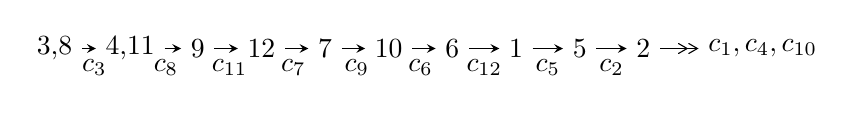
\begin{tikzpicture}[x=23pt, y=7pt]
	% node
	\node (A0) at (-1/8, 0) {3,8};
	\node (A1) at (17/16, 0) {4,11};
	\node (A2) at (17/8, 0) {9};
	\node (A3) at (25/8, 0) {12};
	\node (A4) at (33/8, 0) {7};
	\node (A5) at (41/8, 0) {10};
	\node (A6) at (49/8, 0) {6};
	\node (A7) at (57/8, 0) {1};
	\node (A8) at (65/8, 0) {5};
	\node (A9) at (73/8, 0) {2};
	\node (C1) at (1/2, -1) {$c_{3}$};
	\node (C2) at (13/8, -1) {$c_{8}$};
	\node (C3) at (21/8, -1) {$c_{11}$};
	\node (C4) at (29/8, -1) {$c_{7}$};
	\node (C5) at (37/8, -1) {$c_{9}$};
	\node (C6) at (45/8, -1) {$c_{6}$};
	\node (C7) at (53/8, -1) {$c_{12}$};
	\node (C8) at (61/8, -1) {$c_{5}$};
	\node (C9) at (69/8, -1) {$c_{2}$};
	\node (A10) at (11, 0) {$c_{1},c_{4},c_{10}$};

	% edge
	\draw[->,>=stealth]	
	(A0) edge (A1) (A1) edge (A2) (A2) edge (A3) (A3) edge (A4) (A4) edge (A5) (A5) edge (A6) (A6) edge (A7) (A7) edge (A8) (A8) edge (A9) ;
	\draw[->>,>={angle 60}]	
	(A9) edge (A10);
\end{tikzpicture} \\ 

\end{tabular} \\

\footnotetext{
The image of knot diagram is generated by the software ``\textbf{Draw programme}" developed by Andrew Bartholomew(\url{http://www.layer8.co.uk/maths/draw/index.htm\#Running-draw}), where we modified some parts for our purpose(\url{https://github.com/CATsTAILs/LinksPainter}).
}\phantom \\ \newline 
\centering \textbf{Ideals for irreducible components\footnotemark of $X_{\text{par}}$} 
 
\begin{align*}
I^u_{1}&=\langle 
7.15195\times10^{399} u^{106}-8.59095\times10^{399} u^{105}+\cdots+3.48006\times10^{400} b-4.32470\times10^{402},\\
\phantom{I^u_{1}}&\phantom{= \langle  }3.78913\times10^{398} u^{106}-5.25909\times10^{398} u^{105}+\cdots+4.09419\times10^{399} a-3.05225\times10^{401},\\
\phantom{I^u_{1}}&\phantom{= \langle  }u^{107}-2 u^{106}+\cdots-512 u+512\rangle \\
I^u_{2}&=\langle 
22 u^2+17 b+2 u+40,\;u^2+a- u+2,\;u^3- u^2+2 u-1\rangle \\
\\
I^v_{1}&=\langle 
a,\;14536 v^8+40690 v^7+\cdots+11959 b+36034,\\
\phantom{I^v_{1}}&\phantom{= \langle  }v^9+3 v^8-2 v^7-9 v^6+11 v^5+25 v^4+6 v^3-2 v^2+3 v+1\rangle \\
\end{align*}
\raggedright * 3 irreducible components of $\dim_{\mathbb{C}}=0$, with total 119 representations.\\
\footnotetext{All coefficients of polynomials are rational numbers. But the coefficients are sometimes approximated in decimal forms when there is not enough margin.}
\newpage
\renewcommand{\arraystretch}{1}
\centering \section*{I. $I^u_{1}= \langle 7.15\times10^{399} u^{106}-8.59\times10^{399} u^{105}+\cdots+3.48\times10^{400} b-4.32\times10^{402},\;3.79\times10^{398} u^{106}-5.26\times10^{398} u^{105}+\cdots+4.09\times10^{399} a-3.05\times10^{401},\;u^{107}-2 u^{106}+\cdots-512 u+512 \rangle$}
\flushleft \textbf{(i) Arc colorings}\\
\begin{tabular}{m{7pt} m{180pt} m{7pt} m{180pt} }
\flushright $a_{3}=$&$\begin{pmatrix}1\\0\end{pmatrix}$ \\
\flushright $a_{8}=$&$\begin{pmatrix}0\\u\end{pmatrix}$ \\
\flushright $a_{4}=$&$\begin{pmatrix}1\\u^2\end{pmatrix}$ \\
\flushright $a_{11}=$&$\begin{pmatrix}-0.0925491 u^{106}+0.128453 u^{105}+\cdots+27.8911 u+74.5508\\-0.205512 u^{106}+0.246862 u^{105}+\cdots+10.0191 u+124.271\end{pmatrix}$ \\
\flushright $a_{9}=$&$\begin{pmatrix}-0.141762 u^{106}+0.160044 u^{105}+\cdots-13.9980 u+76.5882\\-0.0579410 u^{106}+0.0583727 u^{105}+\cdots-24.6379 u+21.0757\end{pmatrix}$ \\
\flushright $a_{12}=$&$\begin{pmatrix}-0.225565 u^{106}+0.289473 u^{105}+\cdots+48.0564 u+157.554\\-0.280106 u^{106}+0.347672 u^{105}+\cdots+48.3843 u+184.903\end{pmatrix}$ \\
\flushright $a_{7}=$&$\begin{pmatrix}u\\u\end{pmatrix}$ \\
\flushright $a_{10}=$&$\begin{pmatrix}-0.192530 u^{106}+0.222762 u^{105}+\cdots-4.85824 u+110.365\\-0.108709 u^{106}+0.121091 u^{105}+\cdots-15.4981 u+54.8520\end{pmatrix}$ \\
\flushright $a_{6}=$&$\begin{pmatrix}0.151786 u^{106}-0.171743 u^{105}+\cdots+15.7215 u-78.5804\\0.00714381 u^{106}-0.00235302 u^{105}+\cdots+22.5669 u+5.72998\end{pmatrix}$ \\
\flushright $a_{1}=$&$\begin{pmatrix}0.0917504 u^{106}-0.139578 u^{105}+\cdots-54.8541 u-83.2245\\-0.0193726 u^{106}+0.0291699 u^{105}+\cdots+7.73340 u+16.5814\end{pmatrix}$ \\
\flushright $a_{5}=$&$\begin{pmatrix}-0.125588 u^{106}+0.200162 u^{105}+\cdots+87.0752 u+122.294\\-0.0338377 u^{106}+0.0605837 u^{105}+\cdots+32.2211 u+39.0699\end{pmatrix}$ \\
\flushright $a_{2}=$&$\begin{pmatrix}0.125588 u^{106}-0.200162 u^{105}+\cdots-87.0752 u-122.294\\-0.0267303 u^{106}+0.0296535 u^{105}+\cdots-5.96052 u+12.9504\end{pmatrix}$\\&\end{tabular}
\flushleft \textbf{(ii) Obstruction class $= -1$}\\~\\
\flushleft \textbf{(iii) Cusp Shapes $= 0.991312 u^{106}-1.30501 u^{105}+\cdots-366.569 u-745.449$}\\~\\
\newpage\renewcommand{\arraystretch}{1}
\flushleft \textbf{(iv) u-Polynomials at the component}\newline \\
\begin{tabular}{m{50pt}|m{274pt}}
Crossings & \hspace{64pt}u-Polynomials at each crossing \\
\hline $$\begin{aligned}c_{1},c_{2},c_{4}\end{aligned}$$&$\begin{aligned}
&u^{107}-11 u^{106}+\cdots- u-1
\end{aligned}$\\
\hline $$\begin{aligned}c_{3},c_{7}\end{aligned}$$&$\begin{aligned}
&u^{107}-2 u^{106}+\cdots-512 u+512
\end{aligned}$\\
\hline $$\begin{aligned}c_{5}\end{aligned}$$&$\begin{aligned}
&u^{107}+2 u^{106}+\cdots-10404 u+2312
\end{aligned}$\\
\hline $$\begin{aligned}c_{6},c_{12}\end{aligned}$$&$\begin{aligned}
&u^{107}+3 u^{106}+\cdots-3 u-1
\end{aligned}$\\
\hline $$\begin{aligned}c_{8},c_{11}\end{aligned}$$&$\begin{aligned}
&u^{107}-5 u^{106}+\cdots-5466 u-289
\end{aligned}$\\
\hline $$\begin{aligned}c_{9}\end{aligned}$$&$\begin{aligned}
&17(17 u^{107}+96 u^{106}+\cdots-2.67194\times10^{8} u+4.35330\times10^{7})
\end{aligned}$\\
\hline $$\begin{aligned}c_{10}\end{aligned}$$&$\begin{aligned}
&17(17 u^{107}+61 u^{106}+\cdots+4.98410\times10^{7} u-2813417)
\end{aligned}$\\
\hline
\end{tabular}\\~\\
\newpage\renewcommand{\arraystretch}{1}
\flushleft \textbf{(v) Riley Polynomials at the component}\newline \\
\begin{tabular}{m{50pt}|m{274pt}}
Crossings & \hspace{64pt}Riley Polynomials at each crossing \\
\hline $$\begin{aligned}c_{1},c_{2},c_{4}\end{aligned}$$&$\begin{aligned}
&y^{107}-99 y^{106}+\cdots-29 y-1
\end{aligned}$\\
\hline $$\begin{aligned}c_{3},c_{7}\end{aligned}$$&$\begin{aligned}
&y^{107}-54 y^{106}+\cdots+7340032 y-262144
\end{aligned}$\\
\hline $$\begin{aligned}c_{5}\end{aligned}$$&$\begin{aligned}
&y^{107}-18 y^{106}+\cdots+277740560 y-5345344
\end{aligned}$\\
\hline $$\begin{aligned}c_{6},c_{12}\end{aligned}$$&$\begin{aligned}
&y^{107}+73 y^{106}+\cdots+55 y-1
\end{aligned}$\\
\hline $$\begin{aligned}c_{8},c_{11}\end{aligned}$$&$\begin{aligned}
&y^{107}-81 y^{106}+\cdots+6093612 y-83521
\end{aligned}$\\
\hline $$\begin{aligned}c_{9}\end{aligned}$$&$\begin{aligned}
&289(289 y^{107}-19076 y^{106}+\cdots+8.77063\times10^{16} y-1.89512\times10^{15})
\end{aligned}$\\
\hline $$\begin{aligned}c_{10}\end{aligned}$$&$\begin{aligned}
&289\\
&\cdot(289 y^{107}-7971 y^{106}+\cdots+1153422073109755 y-7915315215889)
\end{aligned}$\\
\hline
\end{tabular}\\~\\
\newpage\flushleft \textbf{(vi) Complex Volumes and Cusp Shapes}
$$\begin{array}{c|c|c}  
\text{Solutions to }I^u_{1}& \I (\text{vol} + \sqrt{-1}CS) & \text{Cusp shape}\\
 \hline 
\begin{aligned}
u &= -0.931265 + 0.406170 I \\
a &= \phantom{-}0.180524 + 0.102775 I \\
b &= -0.628756 + 1.070630 I\end{aligned}
 & -2.30486 + 1.44330 I & \phantom{-0.000000 } 0 \\ \hline\begin{aligned}
u &= -0.931265 - 0.406170 I \\
a &= \phantom{-}0.180524 - 0.102775 I \\
b &= -0.628756 - 1.070630 I\end{aligned}
 & -2.30486 - 1.44330 I & \phantom{-0.000000 } 0 \\ \hline\begin{aligned}
u &= \phantom{-}0.976707 + 0.115936 I \\
a &= \phantom{-}0.599235 + 0.941304 I \\
b &= \phantom{-}0.698962 - 0.236650 I\end{aligned}
 & -3.84509 + 1.95256 I & \phantom{-0.000000 } 0 \\ \hline\begin{aligned}
u &= \phantom{-}0.976707 - 0.115936 I \\
a &= \phantom{-}0.599235 - 0.941304 I \\
b &= \phantom{-}0.698962 + 0.236650 I\end{aligned}
 & -3.84509 - 1.95256 I & \phantom{-0.000000 } 0 \\ \hline\begin{aligned}
u &= -0.356416 + 0.955461 I \\
a &= -0.592799 + 0.220178 I \\
b &= -0.938545 + 0.461272 I\end{aligned}
 & -1.66924 - 1.97469 I & \phantom{-0.000000 } 0 \\ \hline\begin{aligned}
u &= -0.356416 - 0.955461 I \\
a &= -0.592799 - 0.220178 I \\
b &= -0.938545 - 0.461272 I\end{aligned}
 & -1.66924 + 1.97469 I & \phantom{-0.000000 } 0 \\ \hline\begin{aligned}
u &= -1.012720 + 0.132824 I \\
a &= \phantom{-}1.54325 + 0.67120 I \\
b &= \phantom{-}2.50954 + 0.63542 I\end{aligned}
 & -7.33756 + 0.07613 I & \phantom{-0.000000 } 0 \\ \hline\begin{aligned}
u &= -1.012720 - 0.132824 I \\
a &= \phantom{-}1.54325 - 0.67120 I \\
b &= \phantom{-}2.50954 - 0.63542 I\end{aligned}
 & -7.33756 - 0.07613 I & \phantom{-0.000000 } 0 \\ \hline\begin{aligned}
u &= -0.971497 + 0.327337 I \\
a &= \phantom{-}1.094850 + 0.029360 I \\
b &= \phantom{-}2.56859 + 0.95662 I\end{aligned}
 & -2.56341 + 2.94691 I & \phantom{-0.000000 } 0 \\ \hline\begin{aligned}
u &= -0.971497 - 0.327337 I \\
a &= \phantom{-}1.094850 - 0.029360 I \\
b &= \phantom{-}2.56859 - 0.95662 I\end{aligned}
 & -2.56341 - 2.94691 I & \phantom{-0.000000 } 0\\
 \hline 
 \end{array}$$\newpage$$\begin{array}{c|c|c}  
\text{Solutions to }I^u_{1}& \I (\text{vol} + \sqrt{-1}CS) & \text{Cusp shape}\\
 \hline 
\begin{aligned}
u &= \phantom{-}0.088254 + 0.953155 I \\
a &= \phantom{-}0.143294 + 1.178500 I \\
b &= \phantom{-}1.132480 - 0.334989 I\end{aligned}
 & -4.79638 + 0.98699 I & \phantom{-0.000000 } 0 \\ \hline\begin{aligned}
u &= \phantom{-}0.088254 - 0.953155 I \\
a &= \phantom{-}0.143294 - 1.178500 I \\
b &= \phantom{-}1.132480 + 0.334989 I\end{aligned}
 & -4.79638 - 0.98699 I & \phantom{-0.000000 } 0 \\ \hline\begin{aligned}
u &= \phantom{-}0.933039 + 0.143215 I \\
a &= -0.494644 - 1.048140 I \\
b &= -0.343321 - 1.127840 I\end{aligned}
 & -3.78091 - 2.99219 I & \phantom{-0.000000 } 0 \\ \hline\begin{aligned}
u &= \phantom{-}0.933039 - 0.143215 I \\
a &= -0.494644 + 1.048140 I \\
b &= -0.343321 + 1.127840 I\end{aligned}
 & -3.78091 + 2.99219 I & \phantom{-0.000000 } 0 \\ \hline\begin{aligned}
u &= -0.431800 + 0.976154 I \\
a &= -0.668560 - 0.913554 I \\
b &= -0.428460 + 0.364883 I\end{aligned}
 & -3.77986 + 4.80948 I & \phantom{-0.000000 } 0 \\ \hline\begin{aligned}
u &= -0.431800 - 0.976154 I \\
a &= -0.668560 + 0.913554 I \\
b &= -0.428460 - 0.364883 I\end{aligned}
 & -3.77986 - 4.80948 I & \phantom{-0.000000 } 0 \\ \hline\begin{aligned}
u &= \phantom{-}0.228518 + 0.892361 I \\
a &= -0.264082 + 0.338861 I \\
b &= \phantom{-}0.70974 + 1.40915 I\end{aligned}
 & -4.76982 - 0.36186 I & \phantom{-0.000000 } 0 \\ \hline\begin{aligned}
u &= \phantom{-}0.228518 - 0.892361 I \\
a &= -0.264082 - 0.338861 I \\
b &= \phantom{-}0.70974 - 1.40915 I\end{aligned}
 & -4.76982 + 0.36186 I & \phantom{-0.000000 } 0 \\ \hline\begin{aligned}
u &= -0.092471 + 1.078070 I \\
a &= -0.44549 + 1.54366 I \\
b &= -0.620069 + 0.456648 I\end{aligned}
 & -9.17182 - 2.19773 I & \phantom{-0.000000 } 0 \\ \hline\begin{aligned}
u &= -0.092471 - 1.078070 I \\
a &= -0.44549 - 1.54366 I \\
b &= -0.620069 - 0.456648 I\end{aligned}
 & -9.17182 + 2.19773 I & \phantom{-0.000000 } 0\\
 \hline 
 \end{array}$$\newpage$$\begin{array}{c|c|c}  
\text{Solutions to }I^u_{1}& \I (\text{vol} + \sqrt{-1}CS) & \text{Cusp shape}\\
 \hline 
\begin{aligned}
u &= \phantom{-}0.889247 + 0.203541 I \\
a &= -1.189030 + 0.430620 I \\
b &= -2.69411 - 0.64847 I\end{aligned}
 & -2.97691 - 0.95326 I & \phantom{-0.000000 } 0 \\ \hline\begin{aligned}
u &= \phantom{-}0.889247 - 0.203541 I \\
a &= -1.189030 - 0.430620 I \\
b &= -2.69411 + 0.64847 I\end{aligned}
 & -2.97691 + 0.95326 I & \phantom{-0.000000 } 0 \\ \hline\begin{aligned}
u &= -0.242919 + 0.867268 I \\
a &= \phantom{-}0.10892 - 1.53983 I \\
b &= \phantom{-}0.090572 + 0.409338 I\end{aligned}
 & -4.39157 - 8.45275 I & \phantom{-0.000000 } 0 \\ \hline\begin{aligned}
u &= -0.242919 - 0.867268 I \\
a &= \phantom{-}0.10892 + 1.53983 I \\
b &= \phantom{-}0.090572 - 0.409338 I\end{aligned}
 & -4.39157 + 8.45275 I & \phantom{-0.000000 } 0 \\ \hline\begin{aligned}
u &= \phantom{-}1.061410 + 0.301435 I \\
a &= -1.53828 - 0.25745 I \\
b &= -2.67895 + 0.02396 I\end{aligned}
 & -6.91732 - 4.41662 I & \phantom{-0.000000 } 0 \\ \hline\begin{aligned}
u &= \phantom{-}1.061410 - 0.301435 I \\
a &= -1.53828 + 0.25745 I \\
b &= -2.67895 - 0.02396 I\end{aligned}
 & -6.91732 + 4.41662 I & \phantom{-0.000000 } 0 \\ \hline\begin{aligned}
u &= \phantom{-}0.304573 + 1.063250 I \\
a &= \phantom{-}0.997292 + 0.520611 I \\
b &= \phantom{-}1.080310 + 0.440969 I\end{aligned}
 & -5.05564 + 5.39819 I & \phantom{-0.000000 } 0 \\ \hline\begin{aligned}
u &= \phantom{-}0.304573 - 1.063250 I \\
a &= \phantom{-}0.997292 - 0.520611 I \\
b &= \phantom{-}1.080310 - 0.440969 I\end{aligned}
 & -5.05564 - 5.39819 I & \phantom{-0.000000 } 0 \\ \hline\begin{aligned}
u &= -0.870663 + 0.176776 I \\
a &= -0.973907 + 0.679642 I \\
b &= -0.531737 - 0.185116 I\end{aligned}
 & -0.72189 + 2.74860 I & \phantom{-0.000000 } 0 \\ \hline\begin{aligned}
u &= -0.870663 - 0.176776 I \\
a &= -0.973907 - 0.679642 I \\
b &= -0.531737 + 0.185116 I\end{aligned}
 & -0.72189 - 2.74860 I & \phantom{-0.000000 } 0\\
 \hline 
 \end{array}$$\newpage$$\begin{array}{c|c|c}  
\text{Solutions to }I^u_{1}& \I (\text{vol} + \sqrt{-1}CS) & \text{Cusp shape}\\
 \hline 
\begin{aligned}
u &= \phantom{-}1.015450 + 0.504665 I \\
a &= -0.241834 - 0.639622 I \\
b &= -0.171049 - 0.300765 I\end{aligned}
 & \phantom{-}1.09835 - 3.92237 I & \phantom{-0.000000 } 0 \\ \hline\begin{aligned}
u &= \phantom{-}1.015450 - 0.504665 I \\
a &= -0.241834 + 0.639622 I \\
b &= -0.171049 + 0.300765 I\end{aligned}
 & \phantom{-}1.09835 + 3.92237 I & \phantom{-0.000000 } 0 \\ \hline\begin{aligned}
u &= \phantom{-}0.526835 + 0.664073 I \\
a &= \phantom{-}0.813713 + 0.084744 I \\
b &= \phantom{-}0.649668 + 0.235899 I\end{aligned}
 & \phantom{-}2.60177 - 0.62792 I & \phantom{-0.000000 } 0 \\ \hline\begin{aligned}
u &= \phantom{-}0.526835 - 0.664073 I \\
a &= \phantom{-}0.813713 - 0.084744 I \\
b &= \phantom{-}0.649668 - 0.235899 I\end{aligned}
 & \phantom{-}2.60177 + 0.62792 I & \phantom{-0.000000 } 0 \\ \hline\begin{aligned}
u &= -1.076720 + 0.464977 I \\
a &= \phantom{-}0.552748 - 0.958127 I \\
b &= \phantom{-}0.796377 - 0.842288 I\end{aligned}
 & -2.37272 + 7.54825 I & \phantom{-0.000000 } 0 \\ \hline\begin{aligned}
u &= -1.076720 - 0.464977 I \\
a &= \phantom{-}0.552748 + 0.958127 I \\
b &= \phantom{-}0.796377 + 0.842288 I\end{aligned}
 & -2.37272 - 7.54825 I & \phantom{-0.000000 } 0 \\ \hline\begin{aligned}
u &= -0.733065 + 0.330340 I \\
a &= \phantom{-}0.064198 - 0.514775 I \\
b &= -0.374792 - 0.363000 I\end{aligned}
 & -0.769990 - 0.237218 I & -8.00000 - 1.04777 I \\ \hline\begin{aligned}
u &= -0.733065 - 0.330340 I \\
a &= \phantom{-}0.064198 + 0.514775 I \\
b &= -0.374792 + 0.363000 I\end{aligned}
 & -0.769990 + 0.237218 I & -8.00000 + 1.04777 I \\ \hline\begin{aligned}
u &= \phantom{-}0.716753 + 0.360053 I \\
a &= -1.124690 + 0.448670 I \\
b &= \phantom{-}3.46273 - 0.61131 I\end{aligned}
 & -3.50386 - 1.66896 I & -16.6348 - 15.7652 I \\ \hline\begin{aligned}
u &= \phantom{-}0.716753 - 0.360053 I \\
a &= -1.124690 - 0.448670 I \\
b &= \phantom{-}3.46273 + 0.61131 I\end{aligned}
 & -3.50386 + 1.66896 I & -16.6348 + 15.7652 I\\
 \hline 
 \end{array}$$\newpage$$\begin{array}{c|c|c}  
\text{Solutions to }I^u_{1}& \I (\text{vol} + \sqrt{-1}CS) & \text{Cusp shape}\\
 \hline 
\begin{aligned}
u &= \phantom{-}0.092779 + 0.786586 I \\
a &= -0.268044 - 1.184120 I \\
b &= -0.075212 + 0.508676 I\end{aligned}
 & \phantom{-}0.99398 + 2.92097 I & -2.14055 - 8.38546 I \\ \hline\begin{aligned}
u &= \phantom{-}0.092779 - 0.786586 I \\
a &= -0.268044 + 1.184120 I \\
b &= -0.075212 - 0.508676 I\end{aligned}
 & \phantom{-}0.99398 - 2.92097 I & -2.14055 + 8.38546 I \\ \hline\begin{aligned}
u &= \phantom{-}0.758308 + 0.133029 I \\
a &= -0.372777 + 0.723023 I \\
b &= \phantom{-}0.63345 + 1.29744 I\end{aligned}
 & -3.58750 + 2.31232 I & -15.8918 - 2.7555 I \\ \hline\begin{aligned}
u &= \phantom{-}0.758308 - 0.133029 I \\
a &= -0.372777 - 0.723023 I \\
b &= \phantom{-}0.63345 - 1.29744 I\end{aligned}
 & -3.58750 - 2.31232 I & -15.8918 + 2.7555 I \\ \hline\begin{aligned}
u &= \phantom{-}0.722730 + 0.161926 I \\
a &= \phantom{-}1.58847 + 0.40979 I \\
b &= \phantom{-}0.337724 - 0.130488 I\end{aligned}
 & -5.80226 - 7.40735 I & -18.9937 + 9.1512 I \\ \hline\begin{aligned}
u &= \phantom{-}0.722730 - 0.161926 I \\
a &= \phantom{-}1.58847 - 0.40979 I \\
b &= \phantom{-}0.337724 + 0.130488 I\end{aligned}
 & -5.80226 + 7.40735 I & -18.9937 - 9.1512 I \\ \hline\begin{aligned}
u &= \phantom{-}1.232030 + 0.307377 I \\
a &= -0.310429 + 0.667179 I \\
b &= \phantom{-}0.154826 - 0.286118 I\end{aligned}
 & -6.76847 - 1.51759 I & \phantom{-0.000000 } 0 \\ \hline\begin{aligned}
u &= \phantom{-}1.232030 - 0.307377 I \\
a &= -0.310429 - 0.667179 I \\
b &= \phantom{-}0.154826 + 0.286118 I\end{aligned}
 & -6.76847 + 1.51759 I & \phantom{-0.000000 } 0 \\ \hline\begin{aligned}
u &= -0.393537 + 0.609625 I \\
a &= -1.165490 + 0.721828 I \\
b &= -0.669946 + 0.274768 I\end{aligned}
 & -0.31883 - 3.28324 I & -5.60431 + 3.66597 I \\ \hline\begin{aligned}
u &= -0.393537 - 0.609625 I \\
a &= -1.165490 - 0.721828 I \\
b &= -0.669946 - 0.274768 I\end{aligned}
 & -0.31883 + 3.28324 I & -5.60431 - 3.66597 I\\
 \hline 
 \end{array}$$\newpage$$\begin{array}{c|c|c}  
\text{Solutions to }I^u_{1}& \I (\text{vol} + \sqrt{-1}CS) & \text{Cusp shape}\\
 \hline 
\begin{aligned}
u &= -1.212990 + 0.397926 I \\
a &= \phantom{-}0.623595 + 0.309847 I \\
b &= -0.39774 - 2.98122 I\end{aligned}
 & -8.99268 + 4.16407 I & \phantom{-0.000000 } 0 \\ \hline\begin{aligned}
u &= -1.212990 - 0.397926 I \\
a &= \phantom{-}0.623595 - 0.309847 I \\
b &= -0.39774 + 2.98122 I\end{aligned}
 & -8.99268 - 4.16407 I & \phantom{-0.000000 } 0 \\ \hline\begin{aligned}
u &= \phantom{-}1.242800 + 0.298457 I \\
a &= \phantom{-}1.168920 + 0.075796 I \\
b &= \phantom{-}2.89703 + 0.03063 I\end{aligned}
 & -9.14754 - 8.24261 I & \phantom{-0.000000 } 0 \\ \hline\begin{aligned}
u &= \phantom{-}1.242800 - 0.298457 I \\
a &= \phantom{-}1.168920 - 0.075796 I \\
b &= \phantom{-}2.89703 - 0.03063 I\end{aligned}
 & -9.14754 + 8.24261 I & \phantom{-0.000000 } 0 \\ \hline\begin{aligned}
u &= -0.141063 + 1.304170 I \\
a &= -0.115873 - 0.757239 I \\
b &= -0.172892 + 0.880125 I\end{aligned}
 & \phantom{-}1.38178 + 2.91494 I & \phantom{-0.000000 } 0 \\ \hline\begin{aligned}
u &= -0.141063 - 1.304170 I \\
a &= -0.115873 + 0.757239 I \\
b &= -0.172892 - 0.880125 I\end{aligned}
 & \phantom{-}1.38178 - 2.91494 I & \phantom{-0.000000 } 0 \\ \hline\begin{aligned}
u &= \phantom{-}1.204720 + 0.538302 I \\
a &= -0.224257 - 0.099675 I \\
b &= \phantom{-}0.245011 + 1.036330 I\end{aligned}
 & -7.84058 - 4.80609 I & \phantom{-0.000000 } 0 \\ \hline\begin{aligned}
u &= \phantom{-}1.204720 - 0.538302 I \\
a &= -0.224257 + 0.099675 I \\
b &= \phantom{-}0.245011 - 1.036330 I\end{aligned}
 & -7.84058 + 4.80609 I & \phantom{-0.000000 } 0 \\ \hline\begin{aligned}
u &= -1.309760 + 0.270121 I \\
a &= \phantom{-}0.371792 + 1.058620 I \\
b &= \phantom{-}0.086820 + 0.488872 I\end{aligned}
 & -10.74750 - 1.26365 I & \phantom{-0.000000 } 0 \\ \hline\begin{aligned}
u &= -1.309760 - 0.270121 I \\
a &= \phantom{-}0.371792 - 1.058620 I \\
b &= \phantom{-}0.086820 - 0.488872 I\end{aligned}
 & -10.74750 + 1.26365 I & \phantom{-0.000000 } 0\\
 \hline 
 \end{array}$$\newpage$$\begin{array}{c|c|c}  
\text{Solutions to }I^u_{1}& \I (\text{vol} + \sqrt{-1}CS) & \text{Cusp shape}\\
 \hline 
\begin{aligned}
u &= \phantom{-}1.271700 + 0.434265 I \\
a &= \phantom{-}0.883155 - 0.416545 I \\
b &= \phantom{-}2.30508 - 0.40191 I\end{aligned}
 & -8.58798 + 4.36356 I & \phantom{-0.000000 } 0 \\ \hline\begin{aligned}
u &= \phantom{-}1.271700 - 0.434265 I \\
a &= \phantom{-}0.883155 + 0.416545 I \\
b &= \phantom{-}2.30508 + 0.40191 I\end{aligned}
 & -8.58798 - 4.36356 I & \phantom{-0.000000 } 0 \\ \hline\begin{aligned}
u &= -1.275970 + 0.428836 I \\
a &= \phantom{-}0.870350 + 0.396090 I \\
b &= \phantom{-}2.57554 - 0.73466 I\end{aligned}
 & -9.07128 + 3.71874 I & \phantom{-0.000000 } 0 \\ \hline\begin{aligned}
u &= -1.275970 - 0.428836 I \\
a &= \phantom{-}0.870350 - 0.396090 I \\
b &= \phantom{-}2.57554 + 0.73466 I\end{aligned}
 & -9.07128 - 3.71874 I & \phantom{-0.000000 } 0 \\ \hline\begin{aligned}
u &= \phantom{-}0.441267 + 1.276080 I \\
a &= \phantom{-}0.010079 - 1.136560 I \\
b &= -0.075031 + 0.587350 I\end{aligned}
 & -10.4011 + 11.2730 I & \phantom{-0.000000 } 0 \\ \hline\begin{aligned}
u &= \phantom{-}0.441267 - 1.276080 I \\
a &= \phantom{-}0.010079 + 1.136560 I \\
b &= -0.075031 - 0.587350 I\end{aligned}
 & -10.4011 - 11.2730 I & \phantom{-0.000000 } 0 \\ \hline\begin{aligned}
u &= -1.230600 + 0.564328 I \\
a &= -1.137020 - 0.087814 I \\
b &= -2.86197 - 0.20383 I\end{aligned}
 & -7.4189 + 13.7965 I & \phantom{-0.000000 } 0 \\ \hline\begin{aligned}
u &= -1.230600 - 0.564328 I \\
a &= -1.137020 + 0.087814 I \\
b &= -2.86197 + 0.20383 I\end{aligned}
 & -7.4189 - 13.7965 I & \phantom{-0.000000 } 0 \\ \hline\begin{aligned}
u &= -1.323420 + 0.286711 I \\
a &= -0.914417 - 0.024510 I \\
b &= -2.58390 + 0.00153 I\end{aligned}
 & -4.18081 + 2.37986 I & \phantom{-0.000000 } 0 \\ \hline\begin{aligned}
u &= -1.323420 - 0.286711 I \\
a &= -0.914417 + 0.024510 I \\
b &= -2.58390 - 0.00153 I\end{aligned}
 & -4.18081 - 2.37986 I & \phantom{-0.000000 } 0\\
 \hline 
 \end{array}$$\newpage$$\begin{array}{c|c|c}  
\text{Solutions to }I^u_{1}& \I (\text{vol} + \sqrt{-1}CS) & \text{Cusp shape}\\
 \hline 
\begin{aligned}
u &= \phantom{-}1.278700 + 0.503687 I \\
a &= -0.908905 + 0.010734 I \\
b &= -2.44601 + 0.82010 I\end{aligned}
 & -8.52536 - 6.22901 I & \phantom{-0.000000 } 0 \\ \hline\begin{aligned}
u &= \phantom{-}1.278700 - 0.503687 I \\
a &= -0.908905 - 0.010734 I \\
b &= -2.44601 - 0.82010 I\end{aligned}
 & -8.52536 + 6.22901 I & \phantom{-0.000000 } 0 \\ \hline\begin{aligned}
u &= -1.232670 + 0.616020 I \\
a &= \phantom{-}0.285190 - 0.632161 I \\
b &= \phantom{-}0.364306 - 0.134856 I\end{aligned}
 & -4.44227 + 7.78550 I & \phantom{-0.000000 } 0 \\ \hline\begin{aligned}
u &= -1.232670 - 0.616020 I \\
a &= \phantom{-}0.285190 + 0.632161 I \\
b &= \phantom{-}0.364306 + 0.134856 I\end{aligned}
 & -4.44227 - 7.78550 I & \phantom{-0.000000 } 0 \\ \hline\begin{aligned}
u &= \phantom{-}1.267260 + 0.549056 I \\
a &= \phantom{-}0.938331 - 0.109314 I \\
b &= \phantom{-}2.60437 - 0.08018 I\end{aligned}
 & -2.55413 - 8.13238 I & \phantom{-0.000000 } 0 \\ \hline\begin{aligned}
u &= \phantom{-}1.267260 - 0.549056 I \\
a &= \phantom{-}0.938331 + 0.109314 I \\
b &= \phantom{-}2.60437 + 0.08018 I\end{aligned}
 & -2.55413 + 8.13238 I & \phantom{-0.000000 } 0 \\ \hline\begin{aligned}
u &= -0.613234\phantom{ +0.000000I} \\
a &= \phantom{-}0.343678\phantom{ +0.000000I} \\
b &= -0.360765\phantom{ +0.000000I}\end{aligned}
 & -0.940432\phantom{ +0.000000I} & -9.73200\phantom{ +0.000000I} \\ \hline\begin{aligned}
u &= -0.429164 + 1.329720 I \\
a &= -0.068472 - 0.921024 I \\
b &= -0.098161 + 0.749867 I\end{aligned}
 & -5.51395 - 5.51248 I & \phantom{-0.000000 } 0 \\ \hline\begin{aligned}
u &= -0.429164 - 1.329720 I \\
a &= -0.068472 + 0.921024 I \\
b &= -0.098161 - 0.749867 I\end{aligned}
 & -5.51395 + 5.51248 I & \phantom{-0.000000 } 0 \\ \hline\begin{aligned}
u &= -0.397402 + 0.438020 I \\
a &= \phantom{-}1.19302 + 1.61741 I \\
b &= \phantom{-}0.57156 + 4.09559 I\end{aligned}
 & -5.90093 - 0.77524 I & -7.20009 - 8.79210 I\\
 \hline 
 \end{array}$$\newpage$$\begin{array}{c|c|c}  
\text{Solutions to }I^u_{1}& \I (\text{vol} + \sqrt{-1}CS) & \text{Cusp shape}\\
 \hline 
\begin{aligned}
u &= -0.397402 - 0.438020 I \\
a &= \phantom{-}1.19302 - 1.61741 I \\
b &= \phantom{-}0.57156 - 4.09559 I\end{aligned}
 & -5.90093 + 0.77524 I & -7.20009 + 8.79210 I \\ \hline\begin{aligned}
u &= \phantom{-}1.349340 + 0.415520 I \\
a &= -1.217360 + 0.693262 I \\
b &= -2.01551 + 0.42109 I\end{aligned}
 & -13.9537 - 2.9601 I & \phantom{-0.000000 } 0 \\ \hline\begin{aligned}
u &= \phantom{-}1.349340 - 0.415520 I \\
a &= -1.217360 - 0.693262 I \\
b &= -2.01551 - 0.42109 I\end{aligned}
 & -13.9537 + 2.9601 I & \phantom{-0.000000 } 0 \\ \hline\begin{aligned}
u &= \phantom{-}1.27824 + 0.62370 I \\
a &= -0.527044 - 0.887663 I \\
b &= -0.860085 - 0.585152 I\end{aligned}
 & -8.16809 - 11.50410 I & \phantom{-0.000000 } 0 \\ \hline\begin{aligned}
u &= \phantom{-}1.27824 - 0.62370 I \\
a &= -0.527044 + 0.887663 I \\
b &= -0.860085 + 0.585152 I\end{aligned}
 & -8.16809 + 11.50410 I & \phantom{-0.000000 } 0 \\ \hline\begin{aligned}
u &= -0.288463 + 0.497708 I \\
a &= \phantom{-}0.665687 - 0.559774 I \\
b &= -0.203916 + 0.598819 I\end{aligned}
 & -0.62747 + 1.89102 I & -3.97049 - 2.88595 I \\ \hline\begin{aligned}
u &= -0.288463 - 0.497708 I \\
a &= \phantom{-}0.665687 + 0.559774 I \\
b &= -0.203916 - 0.598819 I\end{aligned}
 & -0.62747 - 1.89102 I & -3.97049 + 2.88595 I \\ \hline\begin{aligned}
u &= -1.33200 + 0.52311 I \\
a &= \phantom{-}1.312210 - 0.185097 I \\
b &= \phantom{-}2.36998 + 0.15644 I\end{aligned}
 & -13.1732 + 7.9062 I & \phantom{-0.000000 } 0 \\ \hline\begin{aligned}
u &= -1.33200 - 0.52311 I \\
a &= \phantom{-}1.312210 + 0.185097 I \\
b &= \phantom{-}2.36998 - 0.15644 I\end{aligned}
 & -13.1732 - 7.9062 I & \phantom{-0.000000 } 0 \\ \hline\begin{aligned}
u &= \phantom{-}0.55234 + 1.32267 I \\
a &= \phantom{-}0.388265 - 0.819153 I \\
b &= \phantom{-}0.481113 + 0.580917 I\end{aligned}
 & -9.67010 - 1.15397 I & \phantom{-0.000000 } 0\\
 \hline 
 \end{array}$$\newpage$$\begin{array}{c|c|c}  
\text{Solutions to }I^u_{1}& \I (\text{vol} + \sqrt{-1}CS) & \text{Cusp shape}\\
 \hline 
\begin{aligned}
u &= \phantom{-}0.55234 - 1.32267 I \\
a &= \phantom{-}0.388265 + 0.819153 I \\
b &= \phantom{-}0.481113 - 0.580917 I\end{aligned}
 & -9.67010 + 1.15397 I & \phantom{-0.000000 } 0 \\ \hline\begin{aligned}
u &= -1.29769 + 0.65667 I \\
a &= -0.767810 - 0.380695 I \\
b &= -2.13616 - 0.22858 I\end{aligned}
 & -6.46600 + 1.47782 I & \phantom{-0.000000 } 0 \\ \hline\begin{aligned}
u &= -1.29769 - 0.65667 I \\
a &= -0.767810 + 0.380695 I \\
b &= -2.13616 + 0.22858 I\end{aligned}
 & -6.46600 - 1.47782 I & \phantom{-0.000000 } 0 \\ \hline\begin{aligned}
u &= \phantom{-}1.31949 + 0.75319 I \\
a &= \phantom{-}1.044930 - 0.147670 I \\
b &= \phantom{-}2.73164 - 0.27623 I\end{aligned}
 & -13.2708 - 18.4610 I & \phantom{-0.000000 } 0 \\ \hline\begin{aligned}
u &= \phantom{-}1.31949 - 0.75319 I \\
a &= \phantom{-}1.044930 + 0.147670 I \\
b &= \phantom{-}2.73164 + 0.27623 I\end{aligned}
 & -13.2708 + 18.4610 I & \phantom{-0.000000 } 0 \\ \hline\begin{aligned}
u &= -1.34268 + 0.75552 I \\
a &= -0.894702 - 0.162317 I \\
b &= -2.54796 - 0.12017 I\end{aligned}
 & -8.5253 + 12.8531 I & \phantom{-0.000000 } 0 \\ \hline\begin{aligned}
u &= -1.34268 - 0.75552 I \\
a &= -0.894702 + 0.162317 I \\
b &= -2.54796 + 0.12017 I\end{aligned}
 & -8.5253 - 12.8531 I & \phantom{-0.000000 } 0 \\ \hline\begin{aligned}
u &= -0.399946 + 0.214162 I \\
a &= \phantom{-}1.30736 + 1.02540 I \\
b &= -0.415975 + 0.038938 I\end{aligned}
 & -1.063250 - 0.043134 I & -7.94611 - 1.24147 I \\ \hline\begin{aligned}
u &= -0.399946 - 0.214162 I \\
a &= \phantom{-}1.30736 - 1.02540 I \\
b &= -0.415975 - 0.038938 I\end{aligned}
 & -1.063250 + 0.043134 I & -7.94611 + 1.24147 I \\ \hline\begin{aligned}
u &= \phantom{-}0.149223 + 0.396575 I \\
a &= \phantom{-}0.01530 + 3.13817 I \\
b &= \phantom{-}0.294661 + 0.448912 I\end{aligned}
 & -4.49140 + 1.51008 I & -9.81598 - 1.55694 I\\
 \hline 
 \end{array}$$\newpage$$\begin{array}{c|c|c}  
\text{Solutions to }I^u_{1}& \I (\text{vol} + \sqrt{-1}CS) & \text{Cusp shape}\\
 \hline 
\begin{aligned}
u &= \phantom{-}0.149223 - 0.396575 I \\
a &= \phantom{-}0.01530 - 3.13817 I \\
b &= \phantom{-}0.294661 - 0.448912 I\end{aligned}
 & -4.49140 - 1.51008 I & -9.81598 + 1.55694 I \\ \hline\begin{aligned}
u &= \phantom{-}1.35595 + 0.81241 I \\
a &= \phantom{-}0.749963 - 0.331925 I \\
b &= \phantom{-}2.15867 - 0.11610 I\end{aligned}
 & -12.32240 - 6.52710 I & \phantom{-0.000000 } 0 \\ \hline\begin{aligned}
u &= \phantom{-}1.35595 - 0.81241 I \\
a &= \phantom{-}0.749963 + 0.331925 I \\
b &= \phantom{-}2.15867 + 0.11610 I\end{aligned}
 & -12.32240 + 6.52710 I & \phantom{-0.000000 } 0 \\ \hline\begin{aligned}
u &= -1.61146 + 0.03604 I \\
a &= -0.948244 - 0.190754 I \\
b &= -2.56392 - 0.11689 I\end{aligned}
 & -18.4193 - 6.1353 I & \phantom{-0.000000 } 0 \\ \hline\begin{aligned}
u &= -1.61146 - 0.03604 I \\
a &= -0.948244 + 0.190754 I \\
b &= -2.56392 + 0.11689 I\end{aligned}
 & -18.4193 + 6.1353 I & \phantom{-0.000000 } 0 \\ \hline\begin{aligned}
u &= \phantom{-}1.65879\phantom{ +0.000000I} \\
a &= \phantom{-}0.839440\phantom{ +0.000000I} \\
b &= \phantom{-}2.53074\phantom{ +0.000000I}\end{aligned}
 & -13.8071\phantom{ +0.000000I} & \phantom{-0.000000 } 0 \\ \hline\begin{aligned}
u &= \phantom{-}0.315785\phantom{ +0.000000I} \\
a &= -2.96408\phantom{ +0.000000I} \\
b &= -4.94665\phantom{ +0.000000I}\end{aligned}
 & -3.02083\phantom{ +0.000000I} & -69.6120\phantom{ +0.000000I}\\
 \hline 
 \end{array}$$\newpage\newpage\renewcommand{\arraystretch}{1}
\centering \section*{II. $I^u_{2}= \langle 22 u^2+17 b+2 u+40,\;u^2+a- u+2,\;u^3- u^2+2 u-1 \rangle$}
\flushleft \textbf{(i) Arc colorings}\\
\begin{tabular}{m{7pt} m{180pt} m{7pt} m{180pt} }
\flushright $a_{3}=$&$\begin{pmatrix}1\\0\end{pmatrix}$ \\
\flushright $a_{8}=$&$\begin{pmatrix}0\\u\end{pmatrix}$ \\
\flushright $a_{4}=$&$\begin{pmatrix}1\\u^2\end{pmatrix}$ \\
\flushright $a_{11}=$&$\begin{pmatrix}- u^2+u-2\\-\frac{22}{17} u^2-\frac{2}{17} u-\frac{40}{17}\end{pmatrix}$ \\
\flushright $a_{9}=$&$\begin{pmatrix}- u^2+u-2\\-\frac{22}{17} u^2+\frac{15}{17} u-\frac{40}{17}\end{pmatrix}$ \\
\flushright $a_{12}=$&$\begin{pmatrix}0\\- u\end{pmatrix}$ \\
\flushright $a_{7}=$&$\begin{pmatrix}u\\u\end{pmatrix}$ \\
\flushright $a_{10}=$&$\begin{pmatrix}-\frac{14}{17} u^2+\frac{8}{17} u-\frac{27}{17}\\-\frac{19}{17} u^2+\frac{6}{17} u-\frac{33}{17}\end{pmatrix}$ \\
\flushright $a_{6}=$&$\begin{pmatrix}u\\u^2- u+1\end{pmatrix}$ \\
\flushright $a_{1}=$&$\begin{pmatrix}- u^2+2 u-1\\u^2-2 u\end{pmatrix}$ \\
\flushright $a_{5}=$&$\begin{pmatrix}u\\u^2- u+1\end{pmatrix}$ \\
\flushright $a_{2}=$&$\begin{pmatrix}u\\- u\end{pmatrix}$\\&\end{tabular}
\flushleft \textbf{(ii) Obstruction class $= 1$}\\~\\
\flushleft \textbf{(iii) Cusp Shapes $= \frac{2667}{289} u^2-\frac{10925}{289} u+\frac{2721}{289}$}\\~\\
\newpage\renewcommand{\arraystretch}{1}
\flushleft \textbf{(iv) u-Polynomials at the component}\newline \\
\begin{tabular}{m{50pt}|m{274pt}}
Crossings & \hspace{64pt}u-Polynomials at each crossing \\
\hline $$\begin{aligned}c_{1},c_{2}\end{aligned}$$&$\begin{aligned}
&u^3+u^2-1
\end{aligned}$\\
\hline $$\begin{aligned}c_{3}\end{aligned}$$&$\begin{aligned}
&u^3- u^2+2 u-1
\end{aligned}$\\
\hline $$\begin{aligned}c_{4}\end{aligned}$$&$\begin{aligned}
&u^3- u^2+1
\end{aligned}$\\
\hline $$\begin{aligned}c_{5}\end{aligned}$$&$\begin{aligned}
&u^3
\end{aligned}$\\
\hline $$\begin{aligned}c_{6}\end{aligned}$$&$\begin{aligned}
&u^3-3 u^2+2 u+1
\end{aligned}$\\
\hline $$\begin{aligned}c_{7}\end{aligned}$$&$\begin{aligned}
&u^3+u^2+2 u+1
\end{aligned}$\\
\hline $$\begin{aligned}c_{8}\end{aligned}$$&$\begin{aligned}
&(u-1)^3
\end{aligned}$\\
\hline $$\begin{aligned}c_{9}\end{aligned}$$&$\begin{aligned}
&17(17 u^3+10 u^2- u-1)
\end{aligned}$\\
\hline $$\begin{aligned}c_{10}\end{aligned}$$&$\begin{aligned}
&17(17 u^3-23 u^2+8 u-1)
\end{aligned}$\\
\hline $$\begin{aligned}c_{11}\end{aligned}$$&$\begin{aligned}
&(u+1)^3
\end{aligned}$\\
\hline $$\begin{aligned}c_{12}\end{aligned}$$&$\begin{aligned}
&u^3+3 u^2+2 u-1
\end{aligned}$\\
\hline
\end{tabular}\\~\\
\newpage\renewcommand{\arraystretch}{1}
\flushleft \textbf{(v) Riley Polynomials at the component}\newline \\
\begin{tabular}{m{50pt}|m{274pt}}
Crossings & \hspace{64pt}Riley Polynomials at each crossing \\
\hline $$\begin{aligned}c_{1},c_{2},c_{4}\end{aligned}$$&$\begin{aligned}
&y^3- y^2+2 y-1
\end{aligned}$\\
\hline $$\begin{aligned}c_{3},c_{7}\end{aligned}$$&$\begin{aligned}
&y^3+3 y^2+2 y-1
\end{aligned}$\\
\hline $$\begin{aligned}c_{5}\end{aligned}$$&$\begin{aligned}
&y^3
\end{aligned}$\\
\hline $$\begin{aligned}c_{6},c_{12}\end{aligned}$$&$\begin{aligned}
&y^3-5 y^2+10 y-1
\end{aligned}$\\
\hline $$\begin{aligned}c_{8},c_{11}\end{aligned}$$&$\begin{aligned}
&(y-1)^3
\end{aligned}$\\
\hline $$\begin{aligned}c_{9}\end{aligned}$$&$\begin{aligned}
&289(289 y^3-134 y^2+21 y-1)
\end{aligned}$\\
\hline $$\begin{aligned}c_{10}\end{aligned}$$&$\begin{aligned}
&289(289 y^3-257 y^2+18 y-1)
\end{aligned}$\\
\hline
\end{tabular}\\~\\
\newpage\flushleft \textbf{(vi) Complex Volumes and Cusp Shapes}
$$\begin{array}{c|c|c}  
\text{Solutions to }I^u_{2}& \I (\text{vol} + \sqrt{-1}CS) & \text{Cusp shape}\\
 \hline 
\begin{aligned}
u &= \phantom{-}0.215080 + 1.307140 I \\
a &= -0.122561 + 0.744862 I \\
b &= -0.226957 - 0.881437 I\end{aligned}
 & \phantom{-}1.37919 - 2.82812 I & -14.0563 - 44.2246 I \\ \hline\begin{aligned}
u &= \phantom{-}0.215080 - 1.307140 I \\
a &= -0.122561 - 0.744862 I \\
b &= -0.226957 + 0.881437 I\end{aligned}
 & \phantom{-}1.37919 + 2.82812 I & -14.0563 + 44.2246 I \\ \hline\begin{aligned}
u &= \phantom{-}0.569840\phantom{ +0.000000I} \\
a &= -1.75488\phantom{ +0.000000I} \\
b &= -2.84020\phantom{ +0.000000I}\end{aligned}
 & -2.75839\phantom{ +0.000000I} & -9.12970\phantom{ +0.000000I}\\
 \hline 
 \end{array}$$\newpage\newpage\renewcommand{\arraystretch}{1}
\centering \section*{III. $I^v_{1}= \langle a,\;14536 v^8+40690 v^7+\cdots+11959 b+36034,\;v^9+3 v^8+\cdots+3 v+1 \rangle$}
\flushleft \textbf{(i) Arc colorings}\\
\begin{tabular}{m{7pt} m{180pt} m{7pt} m{180pt} }
\flushright $a_{3}=$&$\begin{pmatrix}1\\0\end{pmatrix}$ \\
\flushright $a_{8}=$&$\begin{pmatrix}v\\0\end{pmatrix}$ \\
\flushright $a_{4}=$&$\begin{pmatrix}1\\0\end{pmatrix}$ \\
\flushright $a_{11}=$&$\begin{pmatrix}0\\-1.21549 v^{8}-3.40246 v^{7}+\cdots-0.204281 v-3.01313\end{pmatrix}$ \\
\flushright $a_{9}=$&$\begin{pmatrix}v\\-0.917468 v^{8}-2.75040 v^{7}+\cdots-1.68777 v-2.76913\end{pmatrix}$ \\
\flushright $a_{12}=$&$\begin{pmatrix}0.298018 v^{8}+0.652061 v^{7}+\cdots-0.483485 v+0.244000\\-0.705410 v^{8}-1.67138 v^{7}+\cdots+2.87842 v-0.490008\end{pmatrix}$ \\
\flushright $a_{7}=$&$\begin{pmatrix}v\\0\end{pmatrix}$ \\
\flushright $a_{10}=$&$\begin{pmatrix}0.109374 v^{8}+0.367255 v^{7}+\cdots+0.0885526 v+0.00200686\\-0.917468 v^{8}-2.75040 v^{7}+\cdots-1.68777 v-2.76913\end{pmatrix}$ \\
\flushright $a_{6}=$&$\begin{pmatrix}-0.120495 v^{8}-0.294506 v^{7}+\cdots+0.670792 v+0.0803579\\0.198846 v^{8}+0.759428 v^{7}+\cdots+1.00962 v-0.427544\end{pmatrix}$ \\
\flushright $a_{1}=$&$\begin{pmatrix}-0.244000 v^{8}-0.433983 v^{7}+\cdots-0.633331 v-0.215486\\-1\end{pmatrix}$ \\
\flushright $a_{5}=$&$\begin{pmatrix}0.244000 v^{8}+0.433983 v^{7}+\cdots+0.633331 v+0.215486\\1\end{pmatrix}$ \\
\flushright $a_{2}=$&$\begin{pmatrix}-0.244000 v^{8}-0.433983 v^{7}+\cdots-0.633331 v+0.784514\\-1\end{pmatrix}$\\&\end{tabular}
\flushleft \textbf{(ii) Obstruction class $= 1$}\\~\\
\flushleft \textbf{(iii) Cusp Shapes $= \frac{30669}{11959} v^8+\frac{76868}{11959} v^7-\frac{100871}{11959} v^6-\frac{237835}{11959} v^5+\frac{437462}{11959} v^4+\frac{579948}{11959} v^3-\frac{66654}{11959} v^2-\frac{147944}{11959} v-\frac{72837}{11959}$}\\~\\
\newpage\renewcommand{\arraystretch}{1}
\flushleft \textbf{(iv) u-Polynomials at the component}\newline \\
\begin{tabular}{m{50pt}|m{274pt}}
Crossings & \hspace{64pt}u-Polynomials at each crossing \\
\hline $$\begin{aligned}c_{1},c_{2}\end{aligned}$$&$\begin{aligned}
&(u-1)^9
\end{aligned}$\\
\hline $$\begin{aligned}c_{3},c_{7}\end{aligned}$$&$\begin{aligned}
&u^9
\end{aligned}$\\
\hline $$\begin{aligned}c_{4}\end{aligned}$$&$\begin{aligned}
&(u+1)^9
\end{aligned}$\\
\hline $$\begin{aligned}c_{5},c_{10}\end{aligned}$$&$\begin{aligned}
&u^9+u^8+2 u^7+u^6+3 u^5+u^4+2 u^3+u-1
\end{aligned}$\\
\hline $$\begin{aligned}c_{6}\end{aligned}$$&$\begin{aligned}
&u^9+3 u^8+8 u^7+13 u^6+17 u^5+17 u^4+12 u^3+6 u^2+u-1
\end{aligned}$\\
\hline $$\begin{aligned}c_{8}\end{aligned}$$&$\begin{aligned}
&u^9+u^8-2 u^7-3 u^6+u^5+3 u^4+2 u^3- u-1
\end{aligned}$\\
\hline $$\begin{aligned}c_{9}\end{aligned}$$&$\begin{aligned}
&u^9+5 u^8+12 u^7+15 u^6+9 u^5- u^4-4 u^3-2 u^2+u+1
\end{aligned}$\\
\hline $$\begin{aligned}c_{11}\end{aligned}$$&$\begin{aligned}
&u^9- u^8-2 u^7+3 u^6+u^5-3 u^4+2 u^3- u+1
\end{aligned}$\\
\hline $$\begin{aligned}c_{12}\end{aligned}$$&$\begin{aligned}
&u^9-3 u^8+8 u^7-13 u^6+17 u^5-17 u^4+12 u^3-6 u^2+u+1
\end{aligned}$\\
\hline
\end{tabular}\\~\\
\newpage\renewcommand{\arraystretch}{1}
\flushleft \textbf{(v) Riley Polynomials at the component}\newline \\
\begin{tabular}{m{50pt}|m{274pt}}
Crossings & \hspace{64pt}Riley Polynomials at each crossing \\
\hline $$\begin{aligned}c_{1},c_{2},c_{4}\end{aligned}$$&$\begin{aligned}
&(y-1)^9
\end{aligned}$\\
\hline $$\begin{aligned}c_{3},c_{7}\end{aligned}$$&$\begin{aligned}
&y^9
\end{aligned}$\\
\hline $$\begin{aligned}c_{5},c_{10}\end{aligned}$$&$\begin{aligned}
&y^9+3 y^8+8 y^7+13 y^6+17 y^5+17 y^4+12 y^3+6 y^2+y-1
\end{aligned}$\\
\hline $$\begin{aligned}c_{6},c_{12}\end{aligned}$$&$\begin{aligned}
&y^9+7 y^8+20 y^7+25 y^6+5 y^5-15 y^4+22 y^2+13 y-1
\end{aligned}$\\
\hline $$\begin{aligned}c_{8},c_{11}\end{aligned}$$&$\begin{aligned}
&y^9-5 y^8+12 y^7-15 y^6+9 y^5+y^4-4 y^3+2 y^2+y-1
\end{aligned}$\\
\hline $$\begin{aligned}c_{9}\end{aligned}$$&$\begin{aligned}
&y^9- y^8+12 y^7-7 y^6+37 y^5+y^4-10 y^2+5 y-1
\end{aligned}$\\
\hline
\end{tabular}\\~\\
\newpage\flushleft \textbf{(vi) Complex Volumes and Cusp Shapes}
$$\begin{array}{c|c|c}  
\text{Solutions to }I^v_{1}& \I (\text{vol} + \sqrt{-1}CS) & \text{Cusp shape}\\
 \hline 
\begin{aligned}
v &= -0.924205 + 0.223068 I \\
a &= \phantom{-0.000000 } 0 \\
b &= -0.037875 + 0.791187 I\end{aligned}
 & -2.26187 + 2.45442 I & -8.53903 - 2.82066 I \\ \hline\begin{aligned}
v &= -0.924205 - 0.223068 I \\
a &= \phantom{-0.000000 } 0 \\
b &= -0.037875 - 0.791187 I\end{aligned}
 & -2.26187 - 2.45442 I & -8.53903 + 2.82066 I \\ \hline\begin{aligned}
v &= \phantom{-}0.295822 + 0.390531 I \\
a &= \phantom{-0.000000 } 0 \\
b &= \phantom{-}0.80973 - 2.39258 I\end{aligned}
 & -6.01628 + 1.33617 I & -16.4774 - 4.4812 I \\ \hline\begin{aligned}
v &= \phantom{-}0.295822 - 0.390531 I \\
a &= \phantom{-0.000000 } 0 \\
b &= \phantom{-}0.80973 + 2.39258 I\end{aligned}
 & -6.01628 - 1.33617 I & -16.4774 + 4.4812 I \\ \hline\begin{aligned}
v &= -0.280601\phantom{ +0.000000I} \\
a &= \phantom{-0.000000 } 0 \\
b &= -2.94345\phantom{ +0.000000I}\end{aligned}
 & -2.84338\phantom{ +0.000000I} & -3.87310\phantom{ +0.000000I} \\ \hline\begin{aligned}
v &= \phantom{-}1.47927 + 0.93319 I \\
a &= \phantom{-0.000000 } 0 \\
b &= -0.218072 + 0.482572 I\end{aligned}
 & \phantom{-}0.13850 + 2.09337 I & -6.02684 - 1.69698 I \\ \hline\begin{aligned}
v &= \phantom{-}1.47927 - 0.93319 I \\
a &= \phantom{-0.000000 } 0 \\
b &= -0.218072 - 0.482572 I\end{aligned}
 & \phantom{-}0.13850 - 2.09337 I & -6.02684 + 1.69698 I \\ \hline\begin{aligned}
v &= -2.21059 + 0.69487 I \\
a &= \phantom{-0.000000 } 0 \\
b &= \phantom{-}0.417942 + 0.357732 I\end{aligned}
 & -5.24306 - 7.08493 I & -9.02021 + 2.94778 I \\ \hline\begin{aligned}
v &= -2.21059 - 0.69487 I \\
a &= \phantom{-0.000000 } 0 \\
b &= \phantom{-}0.417942 - 0.357732 I\end{aligned}
 & -5.24306 + 7.08493 I & -9.02021 - 2.94778 I\\
 \hline 
 \end{array}$$\newpage
\newpage\renewcommand{\arraystretch}{1}
\centering \section*{ IV. u-Polynomials}
\begin{tabular}{m{50pt}|m{274pt}}
Crossings & \hspace{64pt}u-Polynomials at each crossing \\
\hline $$\begin{aligned}c_{1},c_{2}\end{aligned}$$&$\begin{aligned}
&((u-1)^9)(u^3+u^2-1)(u^{107}-11 u^{106}+\cdots- u-1)
\end{aligned}$\\
\hline $$\begin{aligned}c_{3}\end{aligned}$$&$\begin{aligned}
&u^9(u^3- u^2+2 u-1)(u^{107}-2 u^{106}+\cdots-512 u+512)
\end{aligned}$\\
\hline $$\begin{aligned}c_{4}\end{aligned}$$&$\begin{aligned}
&((u+1)^9)(u^3- u^2+1)(u^{107}-11 u^{106}+\cdots- u-1)
\end{aligned}$\\
\hline $$\begin{aligned}c_{5}\end{aligned}$$&$\begin{aligned}
&u^3(u^9+u^8+2 u^7+u^6+3 u^5+u^4+2 u^3+u-1)\\
&\cdot(u^{107}+2 u^{106}+\cdots-10404 u+2312)
\end{aligned}$\\
\hline $$\begin{aligned}c_{6}\end{aligned}$$&$\begin{aligned}
&(u^3-3 u^2+2 u+1)\\
&\cdot(u^9+3 u^8+8 u^7+13 u^6+17 u^5+17 u^4+12 u^3+6 u^2+u-1)\\
&\cdot(u^{107}+3 u^{106}+\cdots-3 u-1)
\end{aligned}$\\
\hline $$\begin{aligned}c_{7}\end{aligned}$$&$\begin{aligned}
&u^9(u^3+u^2+2 u+1)(u^{107}-2 u^{106}+\cdots-512 u+512)
\end{aligned}$\\
\hline $$\begin{aligned}c_{8}\end{aligned}$$&$\begin{aligned}
&(u-1)^3(u^9+u^8-2 u^7-3 u^6+u^5+3 u^4+2 u^3- u-1)\\
&\cdot(u^{107}-5 u^{106}+\cdots-5466 u-289)
\end{aligned}$\\
\hline $$\begin{aligned}c_{9}\end{aligned}$$&$\begin{aligned}
&289(17 u^3+10 u^2- u-1)\\
&\cdot(u^9+5 u^8+12 u^7+15 u^6+9 u^5- u^4-4 u^3-2 u^2+u+1)\\
&\cdot(17 u^{107}+96 u^{106}+\cdots-267194040 u+43532959)
\end{aligned}$\\
\hline $$\begin{aligned}c_{10}\end{aligned}$$&$\begin{aligned}
&289(17 u^3-23 u^2+8 u-1)(u^9+u^8+\cdots+u-1)\\
&\cdot(17 u^{107}+61 u^{106}+\cdots+49840983 u-2813417)
\end{aligned}$\\
\hline $$\begin{aligned}c_{11}\end{aligned}$$&$\begin{aligned}
&(u+1)^3(u^9- u^8-2 u^7+3 u^6+u^5-3 u^4+2 u^3- u+1)\\
&\cdot(u^{107}-5 u^{106}+\cdots-5466 u-289)
\end{aligned}$\\
\hline $$\begin{aligned}c_{12}\end{aligned}$$&$\begin{aligned}
&(u^3+3 u^2+2 u-1)\\
&\cdot(u^9-3 u^8+8 u^7-13 u^6+17 u^5-17 u^4+12 u^3-6 u^2+u+1)\\
&\cdot(u^{107}+3 u^{106}+\cdots-3 u-1)
\end{aligned}$\\
\hline
\end{tabular}\newpage\renewcommand{\arraystretch}{1}
\centering \section*{ V. Riley Polynomials}
\begin{tabular}{m{50pt}|m{274pt}}
Crossings & \hspace{64pt}Riley Polynomials at each crossing \\
\hline $$\begin{aligned}c_{1},c_{2},c_{4}\end{aligned}$$&$\begin{aligned}
&((y-1)^9)(y^3- y^2+2 y-1)(y^{107}-99 y^{106}+\cdots-29 y-1)
\end{aligned}$\\
\hline $$\begin{aligned}c_{3},c_{7}\end{aligned}$$&$\begin{aligned}
&y^9(y^3+3 y^2+2 y-1)(y^{107}-54 y^{106}+\cdots+7340032 y-262144)
\end{aligned}$\\
\hline $$\begin{aligned}c_{5}\end{aligned}$$&$\begin{aligned}
&y^3(y^9+3 y^8+8 y^7+13 y^6+17 y^5+17 y^4+12 y^3+6 y^2+y-1)\\
&\cdot(y^{107}-18 y^{106}+\cdots+277740560 y-5345344)
\end{aligned}$\\
\hline $$\begin{aligned}c_{6},c_{12}\end{aligned}$$&$\begin{aligned}
&(y^3-5 y^2+10 y-1)\\
&\cdot(y^9+7 y^8+20 y^7+25 y^6+5 y^5-15 y^4+22 y^2+13 y-1)\\
&\cdot(y^{107}+73 y^{106}+\cdots+55 y-1)
\end{aligned}$\\
\hline $$\begin{aligned}c_{8},c_{11}\end{aligned}$$&$\begin{aligned}
&(y-1)^3(y^9-5 y^8+12 y^7-15 y^6+9 y^5+y^4-4 y^3+2 y^2+y-1)\\
&\cdot(y^{107}-81 y^{106}+\cdots+6093612 y-83521)
\end{aligned}$\\
\hline $$\begin{aligned}c_{9}\end{aligned}$$&$\begin{aligned}
&83521(289 y^3-134 y^2+21 y-1)\\
&\cdot(y^9- y^8+12 y^7-7 y^6+37 y^5+y^4-10 y^2+5 y-1)\\
&\cdot(289 y^{107}-1.91\times10^{4} y^{106}+\cdots+8.77\times10^{16} y-1.90\times10^{15})
\end{aligned}$\\
\hline $$\begin{aligned}c_{10}\end{aligned}$$&$\begin{aligned}
&83521(289 y^3-257 y^2+18 y-1)\\
&\cdot(y^9+3 y^8+8 y^7+13 y^6+17 y^5+17 y^4+12 y^3+6 y^2+y-1)\\
&\cdot(289 y^{107}-7971 y^{106}+\cdots+1153422073109755 y-7915315215889)
\end{aligned}$\\
\hline
\end{tabular}
\vskip 2pc
\end{document}